\pagebreak

\section{Vincoli}
\label{sez:vincoli}

\subsection{Vincoli tecnologici}
\label{subsec:vincoli-tecnologici}

L’azienda ha definito una serie di vincoli tecnologici per la realizzazione del progetto, al fine di garantire standard qualitativi elevati e l’adozione di pratiche consolidate.\\
Questi vincoli sono essenziali per assicurare l’integrazione con l’ecosistema tecnologico esistente e per sfruttare al meglio le competenze aziendali.\\

\noindent Di seguito vengono descritti nel dettaglio:
\begin{itemize}
    \item \textbf{Documentazione \textit{Swagger} delle \gls{api}:} Ogni \gls{api} sviluppata dovrà essere accompagnata da una documentazione completa generata con \textit{Swagger}. \\
    Questo strumento consente di definire e visualizzare la struttura delle \gls{api-restful}, garantendo una comunicazione chiara e standardizzata tra i diversi \textit{team} di sviluppo;
    \item \textbf{\textit{Test} di unità:} È necessario implementare \textit{test} di unità per tutte le componenti del sistema, sia \gls{frontend} che \gls{backend},
    al fine di garantire la correttezza funzionale del codice e ridurre i rischi di regressioni durante le fasi di sviluppo e manutenzione;
    \item \textbf{Ambiente di \textit{test} funzionante:} La \textit{web application} deve essere operativa in un ambiente di \textit{test} che simuli condizioni reali. \\
    Questo è fondamentale per individuare eventuali problematiche prima del rilascio in produzione;
    \item \textbf{Tecnologie \gls{frontend}:} Nel \gls{frontend} è obbligatorio l’utilizzo di \textit{React.js}, un \textit{framework JavaScript} moderno che garantisce alta modularità e performance, e della libreria \textit{Material-UI} per la progettazione di interfacce utente coerenti e responsivi. \\
    Questi strumenti permettono di sviluppare applicazioni altamente interattive con una \textit{user experience} avanzata;
    \item \textbf{Autenticazione:} Per la gestione dell’autenticazione e autorizzazione, devono essere utilizzati \textit{AWS Amplify} e \textit{AWS Cognito}, soluzioni che offrono sicurezza, scalabilità e facilità di integrazione con altre piattaforme \gls{aws}.
    \item \textbf{Tecnologie \gls{backend}:} Nel \gls{backend}, lo sviluppo deve avvenire utilizzando \textit{NestJS}, un framework basato su \textit{Node.js} che favorisce la creazione di architetture scalabili e modulari. \\
    È inoltre obbligatorio andare ad implementare \gls{api-restful}, aderendo ai principi \textit{REST} per garantire interoperabilità e riusabilità dei servizi;
    \item \textbf{Gestione dei documenti:} La generazione dei documenti deve essere effettuata utilizzando \textit{AWS Bedrock}, una piattaforma innovativa che sfrutta modelli di \gls{ai} per la creazione e l’elaborazione automatizzata di contenuti altamente personalizzati. \\
    I documenti generati devono essere archiviati in modo sicuro nel \textit{cloud} tramite \textit{AWS S3}, che garantisce alta durabilità, scalabilità e accessibilità globale;
    \pagebreak
    \item \textbf{\textit{Database}:} Come \textit{database} per il progetto è richiesto l’uso di \textit{MongoDB}, un \textit{database} \textit{NoSQL} scalabile e flessibile che consente di memorizzare dati in formato \textit{JSON-like}. \\
    Questa scelta permette di gestire facilmente dati non strutturati o semi-strutturati e garantisce alte prestazioni per le operazioni di lettura e scrittura.\\
\end{itemize}

\noindent Questi vincoli tecnologici rappresentano le linee guida principali per lo sviluppo del progetto, promuovendo l’uso di tecnologie all’avanguardia e l’adozione di metodologie che assicurano la qualità e l’efficienza del prodotto finale.

\subsection{Vincoli organizzativi}
\label{subsec:vincoli-organizzativi}

L’organizzazione del lavoro ha seguito precise linee guida per garantire un’efficace gestione del progetto ed una comunicazione fluida tra i vari attori coinvolti.\\

\noindent Di seguito vengono illustrati i vincoli organizzativi imposti dall'azienda:

\begin{itemize}
    \item \textbf{Creazione di \gls{user-stories}:} Durante l'attività di analisi, è necessario andare a creare \gls{user-stories} che descrivano i requisiti del sistema dal punto di vista dell’utente.\\
    Ogni \textit{user story} deve includere una descrizione, i criteri di accettazione ed una priorità.
    Tali \textit{user stories} devono essere tracciate su \textit{Jira}.\\
    Per una descrizione più dettagliata delle \gls{user-stories}, si rimanda alla \hyperref[subsec:user-story-mapping]{sezione §3.2.1};
    \item \textbf{Comunicazione interna tramite \textit{Slack}:} Per le interazioni con il \textit{tutor} aziendale e altre figure aziendali, è richiesto l’uso di \textit{Slack} come strumento di comunicazione.\\
    La piattaforma consente di organizzare discussioni in canali tematici e mantenere una cronologia facilmente accessibile;
    \item \textbf{Lavoro a \gls{sprint}:} Il lavoro è suddiviso in \gls{sprint}, ovvero brevi cicli di sviluppo della durata di una settimana.\\
    Uno \gls{sprint} rappresenta un periodo di tempo delimitato durante il quale il \textit{team} lavora per completare un insieme di obiettivi predefiniti, spesso basati su specifiche \textit{user stories}. \\
    Ogni \gls{sprint} inizia con una pianificazione, dove vengono definiti i compiti prioritari da completare, e termina con una \textit{sprint retrospective}, 
    una riunione durante la quale il \textit{team} analizza i risultati ottenuti, identifica eventuali problematiche e propone soluzioni per migliorare i successivi \gls{sprint}. \\
    Questo approccio garantisce un processo di sviluppo iterativo e incrementale, promuovendo la consegna continua di valore;
    \item \textbf{Utilizzo di \gls{git-flow}:} Durante lo stage, il lavoro di sviluppo sarà organizzato utilizzando \gls{git-flow}, una metodologia di gestione del flusso di lavoro in \textit{Git} che aiuta a strutturare in modo efficiente i processi di sviluppo e gestione del codice sorgente\footcite{site:git-flow}.\\
    \gls{git-flow} si basa su un ramo principale (\texttt{main}) e due rami di sviluppo principali: \texttt{develop} per lo sviluppo quotidiano e \texttt{feature} per le nuove funzionalità.\\
    Inoltre, vengono utilizzati rami di \texttt{release} per preparare nuove versioni stabili del \textit{software} e rami di \texttt{hotfix} per correggere errori urgenti nelle versioni di produzione.
    Il flusso di lavoro con \gls{git-flow} permette di isolare le modifiche, garantire che il codice sia sempre testato e pronto per essere distribuito, e facilitare il lavoro in \textit{team}, mantenendo il codice principale sempre stabile.\\
    Ogni modifica al codice viene effettuata su rami specifici, evitando conflitti e semplificando il processo di fusione (\textit{merge}) delle modifiche;
    \item \textbf{Comunicazione costante con il \textit{tutor} aziendale:} Sono previsti \textit{meeting} settimanali con il \textit{tutor} aziendale per effettuare la \textit{sprint retrospective}, discutere i progressi ed affrontare eventuali problematiche.\\
    Qualsiasi difficoltà o dubbio deve essere comunicato tempestivamente per garantire un supporto immediato e risolvere le criticità in modo efficace;
    \item \textbf{Comunicazione costante con il Relatore:} È richiesta una comunicazione regolare con il relatore ogni cinque giorni lavorativi per fornire aggiornamenti sullo stato di avanzamento, verificare il rispetto del Piano di Lavoro e dare una pianificazione riguardo al periodo successivo.\\
\end{itemize}

\noindent Questi vincoli organizzativi sono stati definiti per facilitare la pianificazione, il monitoraggio e l’esecuzione del progetto, promuovendo un ambiente di lavoro ben strutturato.

\subsection{Vincoli alla progettazione e a alla codifica}

La scelta delle tecnologie utilizzate nel progetto è stata in gran parte imposta dall'azienda.\\
In particolare, l'azienda ha imposto l'adozione di \textit{ReactJS} come \textit{framework} per il \gls{frontend}, di \textit{NestJS} per il \gls{backend} e di \textit{MongoDB} come \textit{database}.\\
Queste scelte sono state motivate da una serie di considerazioni interne, tra cui la familiarità aziendale con le tecnologie e la loro capacità di soddisfare le esigenze di scalabilità e manutenibilità del progetto.\\

\noindent Inoltre, l'azienda ha imposto l'utilizzo di una serie di servizi \gls{aws} per la gestione dell'autenticazione, la generazione dei progetti e il salvataggio dei documenti.\\
Questi sono stati ampiamente discussi nella {\hyperref[sez:tecnologie-sviluppo]{Sezione 1.4}} relativa alle tecnologie di sviluppo.


\subsection{Scelta del LLM}
\label{subsec:scelta-llm}

La scelta del \gls{llm} più adatto per la generazione dei progetti è stata un passo cruciale nel processo di sviluppo, poiché il modello scelto avrebbe influenzato significativamente la qualità e la coerenza dei contenuti generati.\\
Durante la fase di valutazione, sono stati considerati diversi modelli di linguaggio avanzati, tra cui \textit{GPT-4}, \textit{Claude 3.5 Sonnet}, \textit{Amazon Titan} e \textit{Llama}, ognuno dei quali dettagliamente descritto nella {\hyperref[subsec:llm-confronto]{Sezione 2.3.2}}.\\

\noindent La decisione finale è stata presa tenendo conto delle specifiche necessità del progetto, in particolare nell'ambito dell'utilizzo di \textit{AWS Bedrock}, la piattaforma scelta per l'integrazione con i modelli di linguaggio.

\subsubsection{Esclusione di GPT-4}

Il modello \textit{GPT-4}, pur essendo uno dei più potenti e avanzati modelli di linguaggio disponibili, è stato scartato a priori.\\
Questa scelta è stata dettata dal fatto che \textit{GPT-4} non è disponibile tramite le \gls{api} di \textit{AWS Bedrock}, la piattaforma utilizzata per la gestione dei modelli nel progetto.\\
Poiché l'architettura del sistema dipendeva fortemente dall'integrazione con \textit{AWS Bedrock}, l'impossibilità di utilizzare \textit{GPT-4} ha automaticamente escluso questo modello dalla selezione.

\subsubsection{Scelta di \textit{Claude 3.5 Sonnet}}

Dopo aver escluso \textit{GPT-4}, la scelta si è concentrata sui tre \gls{llm} rimanenti: \textit{Claude 3.5 Sonnet}, \textit{Amazon Titan} e \textit{Llama}. \\
Dopo una serie di valutazioni, discussioni con il \textit{tutor} aziendale e approfondimenti sulle caratteristiche dei modelli, la decisione finale è ricaduta su \textit{Claude 3.5 Sonnet} di \textit{Anthropic}.\\

\noindent La scelta di \textit{Claude 3.5 Sonnet} è stata motivata principalmente dalla sua capacità di generare testi molto lunghi, una caratteristica fondamentale per il progetto, che prevedeva la generazione di progetti molto dettagliati.\\
A differenza di altri modelli, che possono essere più efficienti nel generare testi brevi e concisi, \textit{Claude 3.5 Sonnet} ha dimostrato di essere in grado di mantenere una coerenza narrativa e una logica fluida anche su testi di grande lunghezza.\\

\noindent Uno dei principali svantaggi in merito alla scelta di \textit{Claude 3.5 Sonnet} è la latenza maggiore che esso comporta, rispetto ad altri modelli più leggeri,
tuttavia questao non ha rappresentato un problema significativo, poiché la generazione dei contenuti è gestita centralmente nel \gls{backend}, dove la latenza può essere gestita in modo più efficiente e non impatta l'esperienza utente finale in modo negativo.\\

\noindent La {\hyperref[fig:sonnet-comparison]{Figura 3.7}} riporta la tabella comparativa contenente l'aggiornamento di \textit{Claude 3.5 Sonnet} rispetto ad altri modelli \gls{llm}.

\begin{figure}[H]
    \centering
    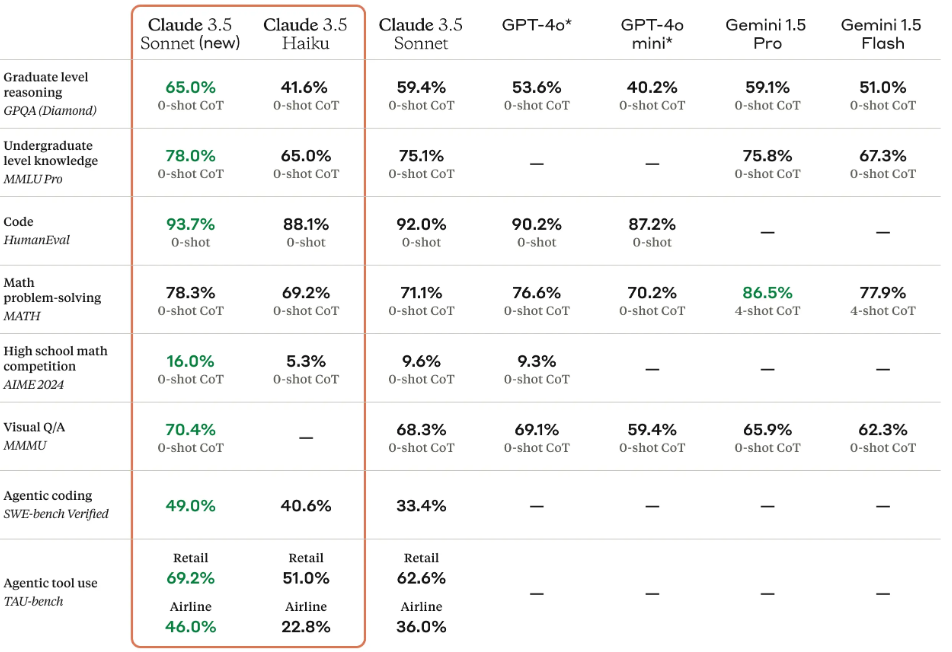
\includegraphics[scale=0.6]{sonnet-comparison.png}
    \caption{Confronto tra \textit{Sonnet} ed altri \gls{llm} - Ottobre 2024}
    \cite{site:updated-sonnet}
    \label{fig:sonnet-comparison}
\end{figure}

\subsection{Prodotti attesi}
\label{subsec:prodotti-attesi}

Il progetto prevede la consegna di diversi prodotti finali che soddisfino i requisiti tecnici e organizzativi stabiliti.\\

\noindent Di seguito vengono elencati e descritti i principali prodotti attesi:

\begin{itemize}
    \item \textbf{\textit{Web application}:} Lo sviluppo di una \textit{web application} completa e funzionante, che consenta agli utenti finali di interagire con le funzionalità previste dal progetto;
    \item \textbf{\gls{api-restful}:} La realizzazione di un set di \gls{api-restful} che fornisca i servizi \gls{backend} necessari per il funzionamento della \textit{web application};
    \item \textbf{Documento di analisi progettuale:} Un documento esaustivo che descriva nel dettaglio le scelte progettuali e i servizi \gls{aws} utilizzati.\\
    Questo documento deve evidenziare il ruolo di ciascun servizio, come \textit{AWS Bedrock} per la generazione di documenti e \textit{AWS S3} per l’archiviazione nel cloud, 
    andando a giustificare le scelte in termini di benefici per il progetto;
    \item \textbf{Documentazione delle \gls{api} con \textit{Swagger}:} È prevista la generazione automatica della documentazione delle \gls{api-restful} tramite \textit{Swagger}. \\
    Tale documentazione deve includere informazioni dettagliate sulle funzionalità disponibili, i percorsi, i metodi supportati, i formati di richiesta e risposta, e gli eventuali codici di errore. \\
    La documentazione deve essere costantemente aggiornata per riflettere eventuali modifiche alle \gls{api};
    \item \textbf{Documentazione del piano di \textit{test}:} Un documento dettagliato che descriva il piano di \textit{test} e collaudo della piattaforma. \\
    Questo piano deve includere le strategie di \textit{test} per tutte le componenti del sistema, comprese le \gls{api-restful}, la \textit{web application} e i servizi \gls{backend}.\\
    La documentazione deve includere i \textit{test} unitari, i \textit{test} di integrazione, i \textit{test} di sistema e i \textit{test} di accettazione. \\
    Ogni \textit{test} dovrà essere accompagnato da un piano di esecuzione e dai criteri di accettazione per garantire la qualità e la funzionalità del sistema in ogni sua parte.\\
\end{itemize}

\noindent Questi prodotti rappresentano il risultato tangibile delle attività di sviluppo e progettazione, garantendo sia la funzionalità tecnica che la trasparenza documentale del progetto.

